\section{General context}
\huge skip ahead to section \cref{ref:foursquare}, I thought we needed to write background and etc.
\normalsize
\newline
{\color{blue}
With harddisks becoming faster, cheaper and more efficient, we are able to store more information than before. Using this information is a a useful way to learn how to optimize businesses. Ships can use information
from their sensors to detect errors before they will happen, businesses can understand their market better, and countless more opportunities exist. Notably, Foursquare was able to predict how many iPhones would be sold based upon user data\cite{predictFoursquare}. The term ``Big Data'' is believed to be coined in 2000 by Diebold in\cite{HistoryOfBigData}, when the world was producing 2 to 3 exabytes per year. Today we produce the same amount of data on a daily basis. Thus, the term ``big data'' can be ambiguous. We tend to refer to it as having to deal with data-sets that are so large that naive approaches are inadequate. This can vary from one case to the other; some are dependent on having data quickly whereas others can spend more time. Therefore some companies might think of gigabytes as having big data whereas others will apply the term to data-sets of petabytes. 

Addressing the challenges of big data, there are today many different frameworks and theories.~\cite{fundamentalsPensum} suggests that there are five different aspects one needs to consider. These are listed in~\Cref{tab:fivev}. In addition,~\cite{someone} postulated that
all solutions in Big Data will have to choose at most two of either consistency, availability or partition tolerance. This is referred to as the CAP theorem.  Even though the author of the cap theorem later published an article saying that the theorem was misleading, it still gives the valuable insight that working with big data will often require making compromises.


\begin{table}
\centering
\begin{tabular}{p{.1\textwidth}|p{.8\textwidth}}
        Volume & Size of the data  \\
        Velocity & The speed of which data is created, accumulated and processed \\
        Variety & Type of source for data (typically heterogeneous) \\
        Veracity & How truth-full data is; can we trust our data sources? What happens if we read one out of
        10 000 sensors indicating a defect?\\
        Value & How useful is the information we acquire? \\
    \end{tabular}
\caption{The five V's of Big Data}
\label{tab:fivev}
\end{table}


This paper outlines a solution where we use the Apache Spark framework to go through some gigabytes of Twitter and Foursquare data-sets. These data-sets are stored using Hadoop File System (HDFS).  Spark is seen by some as the successor of Hadoop MapReduce. The latter framework was introduced in 2004\cite{mapReduce2004} whereas spark was introduced in 2014.  Spark has been proven to work up to 10 times faster on disk than MapReduce, and 100 times faster in memory. This is in part because of more efficient usage of memory, and concepts like resilient distributed data-sets (RDD), capable of efficiently computing subsets of data that are resilient to crashes. Also, one can operate on  RDD's  with lazy functions. This allows Spark to compute graphs of operations before any action is taken on a data-set. This means that iterative operations in Spark may avoid penalties taken in other frameworks, like MapReduce, where data is shuffled excess times to operations sequentially.


\section{Overview of paper}

The challenge we address is that of finding an efficient solution to our problems. Naive approaches 
to big-data solutions may  exhaust memory-resources or take too long for them to be feasible. To mitigate this, we use concepts of caching, broadcasting RDD's and try to use narrow dependencies rather than wide whenever possible.

We use PySpark, the python API for Spark. To make the results general, we will not explore performance optimizations regarding size of partitions or memory usage; we write code as if we have infinite memory. This means choosing greedy caching options when possible.
All solutions run at a single computer. It has an AMD quad-core processor running 64-bit Linux kernel 4.4 on 8 GB of memory. The harddisks are two solid state drives with RAID 0 (striping). Output from benchmarks are done using wall-clock time with python's ``time'' module. This makes the timing result prone to numerous sources of error, however, it should still be able to highlight critical differences between algorithmic approaches.
}

\section{Foursquare Analysis}\label{ref:foursquare}
The next subsections will look over our solutions for problem assignments for a data-set from Foursquare. The data-set is 1.8 GB (19265257 lines) of tab-separated data and a header-row with column names. For all sub-tasks we start by mapping the input by their columns (splitting on a tab) and filtering out the header. This is done lazily, so the run-time cost of doing this is included in the computation for each sub-task. Also, in order to assess the output 
we need to perform an action on the RDD\.  In the majority of the cases this will involve writing 
output to disk. An alternative approach would be to run the method ``\textit{collect}'' which executes all pending operations on the RDD and copies all output to memory. However, writing to disk is easier in terms of memory management and makes it easier to verify outputs are correct.


\subsection{Iterating Over a Large Data-set: What Time is It?}\label{sec:iterate}
Our first assignment is iterating over a large data-set, folding together a timestamp and offset to produce a single datetime that is local to our own timezone. There are two important considerations to make: whether or not to cache the data-set first, and the cost of our folding operation. Regarding the latter, we write a lambda using standard libraries from Python, which should be reasonably fast, although other implementations in for example Scala might have performed better. 
For the former case of caching vs no caching, we let the wall clock decide for us: we ran the same
computations twice and compare them in \Cref{tab:cacheVsNoCacheFold}. 

\begin{table}[Hb]
\centering
\begin{tabular}{p{.17\textwidth}|p{.3\textwidth}}
        With Caching & 473 seconds \\
        Without Caching & 501 seconds\\
    \end{tabular}
    \caption{The difference from a cached and non-cached run for task~\ref{sec:iterate}}
\label{tab:cacheVsNoCacheFold}
\end{table}

\lstset{language=Python,caption={Source code for code in task 2}}
\lstinputlisting[language=Python, firstline=12, lastline=14]{src/code.py}

\subsection{Simultaneously Iterating over Heterogeneous Data-sets: Where are We Located?}\label{sec:where}
Each checkin in Foursquare has a latitude and longitude. These can be mapped to find closest
city that the check-ins occurred in.  We need to pinpoint locations to a fixed list of cities 
in order to be able to decide statistics regarding regions. 

Spark doesn't allow you to simultaneously iterate multiple \textit{writable} RDD's. However, you can \textit{broadcast} them, making them read-only. In read-only form, you can cache the RDD efficiently and share them across nodes. One of the reasons it is only permitted to do so only  in read-only is to ensure data consistency: each node must receive the same data. 

Unlike \Cref{sec:iterate}, the lambda function we pass to map between coordinates (latitude and longitude) is now more critical. Computing distance between two sets of coordinates is an expensive operation, making implementation details critical. The work of~\cite{mackey2010efficient} shows more than roughly 40\% speed improvement for optimized coordinate-mapping functions. However, as we are not too interested in benchmarking pythonic functions we still use a simpler and more general haversine formula.

More critical, big-data related factors involve \textit{filterting}. We therefore apply a radius-filtering on all cities to avoid calculating the score for each one. We also show the effect of broadcasting and its impact on performance.
We wanted to make use of an efficient data-structure called the K-D tree, giving O~(log $n$) search time for a set of coordinates. While the data-structure gives a good filtering of coordinates, it is worth noting that it cannot be broadcast with Spark, which makes look-ups difficult to code and use across clusters. Therefore the code did not work (without tampering too much). I provide the non-working code anyway for kd-trees  in ``task3.py''. The executions and their output times are given in~\Cref{tab:task3out}.

\begin{table}
\centering
\begin{tabular}{p{.30\textwidth}|p{.4\textwidth}}
        Without caching & 3331 seconds\\
        Without caching, broadcast  & 3343 seconds \\
        Cached, no broadcasting & 3444 seconds \\
        Cached, broadcast  & 3472  seconds \\
    \end{tabular}
    \caption{Execution times for the different approaches in~\Cref{sec:where}}
\label{tab:task3out}
\end{table}

The results may come as a surprise to some. However, it is worth noting that we only iterate over the data once or twice, which is why caching doesn't provide a speedup. Broadcasting the variables also means sharing it across all nodes, but when we only have 400 entries which we also filter, we find in this case that the initial cost of broadcasting slows the program down.

\lstset{language=Python,caption={Source code for code in task 3}}
\lstinputlisting[language=Python, firstline=32, lastline=51]{src/code3.py}

\subsection{How Many Unique Users: Counting Distinct Keys}\label{sec:distinct}
There aren't that many approaches for finding the number of unique users.
We simply execute a map for the column we are interested in, and the amount of 
distinct rows that are left. This took about 70 seconds. The result was 256307.

\lstset{language=Python,caption={Source code for code in task 4a}}
\lstinputlisting[language=Python, firstline=19, lastline=22]{src/code.py}

\subsection{How Many Unique Users: Counting Distinct Keys \textit{and their Occurrences}}\label{sec:uniqueUsers}
%task 4b
This task is similar to~\Cref{sec:distinct}, except we need to show the actual amount of occurrences for each distinct key. Spark provides a ``\textit{countByValue~()}'' which does this for us. However, writing a large python-dictionary to disk is not too efficient. Therefore, we use a map to append a number to all entries in the tuples, and do a ``\textit{countByValue~()}'', before we save to disk.  This takes 117 seconds.

\lstset{language=Python,caption={Source code for code in task 4b}}
\lstinputlisting[language=Python, firstline=31, lastline=35]{src/code.py}

\subsection{How Many Check-ins: Counting Length of Data-sets}
%task 4c
When a task is simple, it is sometimes easy to try to optimize it. However, any python function
will be slower than simply executing a ``\textit{count~()}'' on the data-set. For ease of programming, we do not avoid trimming the header (which could save some computation time). The result is that there were 19265256 users.
We did not cache the data before executing count, as we are only doing one pass.

\lstset{language=Python,caption={Source code for code in task 4c}}
\lstinputlisting[language=Python, firstline=43, lastline=46]{src/code.py}

\subsection{How Many Countries: Filtering RDD's}\label{sec:countries}
% task 4d
This task is similar to \Cref{sec:where}, however, we would like to apply one more transformation on the input: filtering to only have distinct countries.
We choose the fastest approach from \Cref{sec:where}, that is, no caching or broadcast, but we apply a ``\textit{distinct~()}'' and ``\textit{count~()}'' in the end (which was the quickest way to get list of distinct keys in \Cref{sec:distinct}). We get 46 countries in 3748 seconds.


\subsection{How Many Cities: Filtering RDD's}
% task 4e
We apply the same logic as in \Cref{sec:countries}, and get our result of
174 cities in 3527 seconds.


\subsection{Length of Session: Folding Values}
%task 5
This task is similar to \Cref{sec:uniqueUsers}, except we are getting session ID as the key. Therefore we apply the same ''\textit{reduceByKey~()}''.

After that we use Spark's ''\textit{histogram~()}'' to get histogram values; data and buckets. We choose monotonically increasing values for the buckets, which according to Spark documentation gives $O(1)$ 
insertion rather
than $O(\log{n})$. As there are significant differences especially around 1,2 and 3 buckets, we want the buckets around the smaller values to be linearly spaced. Linearly spaced buckets create many empty slots for numbers higher than 100 check-ins, so we use logarithmic scaling on both axes to make the numbers more meaningful. The result is in \Cref{fig:histogram}. Notably, there are no users with only 1 checkin. We also see a stable trend with roughly decreasing amount of check-ins and users, which makes sense intuitively.

\begin{figure}
    \centering
    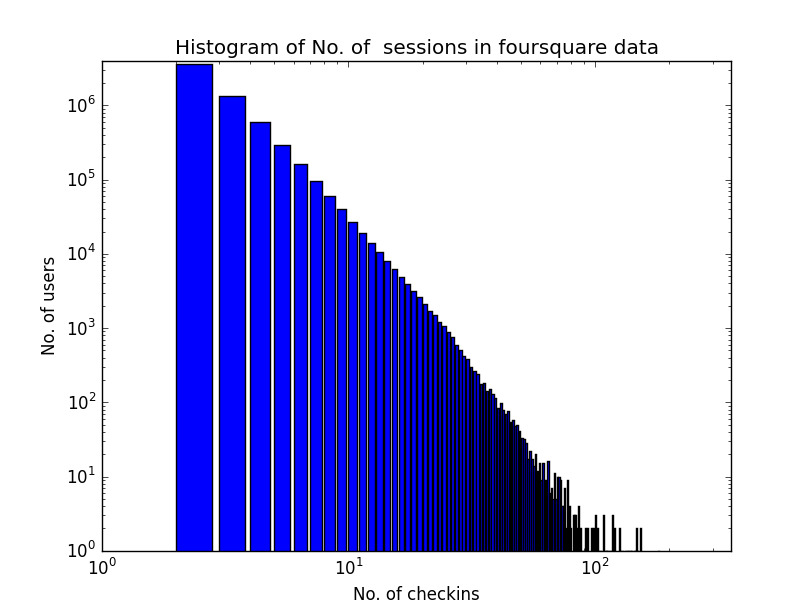
\includegraphics[height=9cm,keepaspectratio]{histogram.jpg}
\caption{Histogram for amount of check-ins per sessions}
\label{fig:histogram}
\end{figure}

\newpage
\lstset{language=Python,caption={Source code for code in task 5}}
\lstinputlisting[language=Python, firstline=74, lastline=79]{src/code.py}

\subsection{Calculating Distance: Folding Values}\label{sec:distanceCalc}
%task 6
In this task, we need to do multiple passes over the dataset. First
we have to filter out sessions with less than 4 check-ins, and then we have to do another pass to calculate length in distance between sessions. 

Assuming that data stays in-order of date, we use a lambda in reduceByKey to combine distances together. ``\textit{reduceByKey~()}'' is quite similar to ``\textit{aggregateByKey~()}'', We try two approaches, each with and without caching the data pre-emptively. Approach \#1 is to first compute the set of of sessions with \textit{less} than 4 check-ins, and then use a reverse set intersection (set $S - $ set $T$) to get the remaining sessions, and calculating their distance. The other is to calculate the number of sessions directly, and then doing a ``\textit{filter~()}'' on the rdd.

We also considered another approach similar to the aggregate function, where we first compute the set of sessions with 4 or more check-ins, broadcast that set, and then iterate the complete data-set, filtering the ones that are too short. This approach, however, was terminated after we discovered it took more than 500 seconds, twice as long the aggregate.
We also did not explore subtractByKey cached, as this was deemed to be too much slower than aggregateByKey anyway. The results are given in~\Cref{tab:aggreagateOrSubtract}

\begin{table}
\centering
\begin{tabular}{p{.29\textwidth}|p{.4\textwidth}}
        Aggregate, not cached & 205 seconds \\
        Aggregate, cached & 299 seconds \\
        Subtract by key, not cached & 942 seconds \\
    \end{tabular}
    \caption{The difference from a cached and non-cached run for task~\ref{sec:iterate}}
\label{tab:aggreagateOrSubtract}
\end{table}

Again, the cached results are slower than not caching which may come as a surprise. However, it is a clear lesson that caching is an expensive operations and will need careful consideration.


\lstset{language=Python,caption={Source code for code in task 5}}
\lstinputlisting[language=Python, firstline=144, lastline=155]{src/code.py}

\subsection{Finding Longest Sessions: Sorting and Filtering Output}
%task 7
In this task, we need to gather sessions that have traveled the furthest.
There are many ways to Rome. We cannot directly fold values by key, since we want retain all check-ins for the key session\_id (it is possible to append them to some large array, but we consider this too messy to go forth with).

Although shown to be in-effective in \Cref{sec:distanceCalc}, we do two computations: first we find all sessions that has a long travel distance. Then, we re-iterate over the data-set, finding each checkin that belongs to our found session-ids. In the end, we write the output to a single file and upload it to cartodb. While not necessarily as fast as aggregating, we finish in 429 seconds, which is acceptable. 
The result can be seen in \Cref{fig:cartoDB}. The link to the map is \url{https://andsild.cartodb.com/viz/081ce90c-0b2a-11e6-937d-0ea31932ec1d/map}.


\begin{figure}
    \centering
    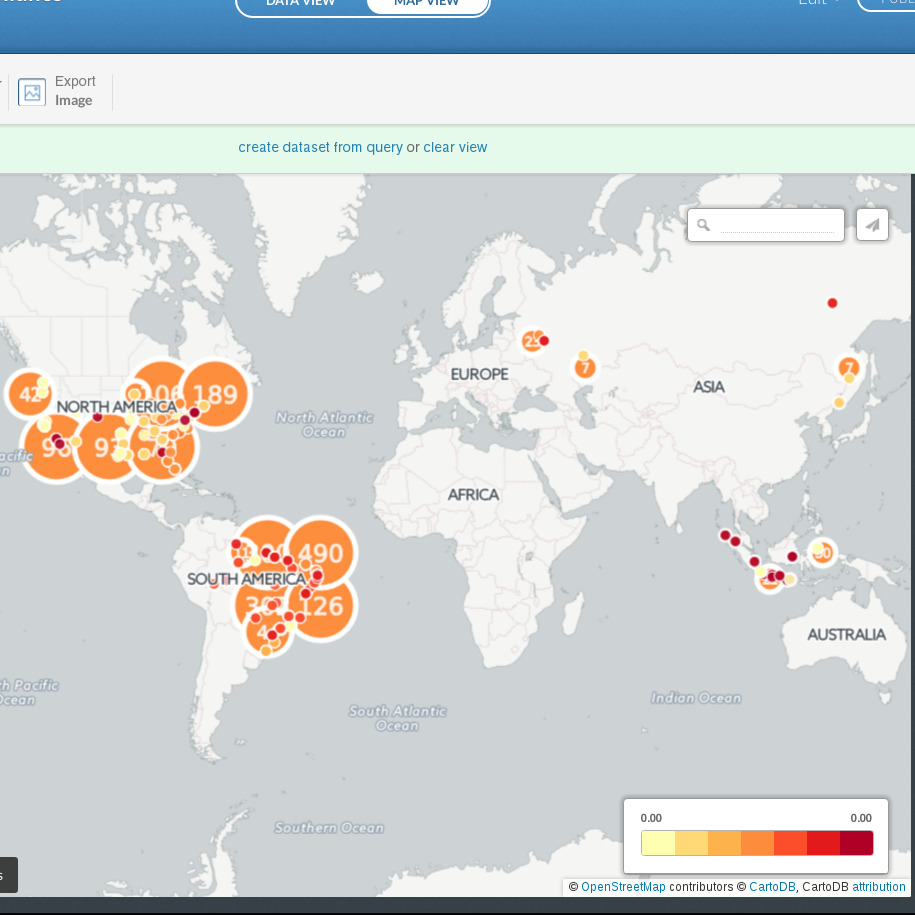
\includegraphics[height=9cm,keepaspectratio]{cartodb.jpg}
\caption{CartoDB result for longest sessions in the foursquare data-set}
\label{fig:cartoDB}
\end{figure}


\lstset{language=Python,caption={Source code for code in task 5}}
\lstinputlisting[language=Python, firstline=171, lastline=183]{src/code.py}

\section{Criticism}
When executing on a smaller data-set (100 MB) there were move vivid differences between
caching and no caching. However, I assume I should benchmark for the large data-set, hence the drawn conclusions.
